%
% $RCSfile: hardware_connection.tex,v $
%
% Copyright (C) 2002-2008. Christian Heller.
%
% Permission is granted to copy, distribute and/or modify this document
% under the terms of the GNU Free Documentation License, Version 1.1 or
% any later version published by the Free Software Foundation; with no
% Invariant Sections, with no Front-Cover Texts and with no Back-Cover
% Texts. A copy of the license is included in the section entitled
% "GNU Free Documentation License".
%
% http://www.cybop.net
% - Cybernetics Oriented Programming -
%
% http://www.resmedicinae.org
% - Information in Medicine -
%
% Version: $Revision: 1.1 $ $Date: 2008-08-19 20:41:07 $ $Author: christian $
% Authors: Christian Heller <christian.heller@tuxtax.de>
%

\subsection{Hardware Connection}
\label{hardware_connection_heading}
\index{Knowledge-Hardware Connection}
\index{Operating System}
\index{OS}
\index{Daemon}
\index{Knowledge}
\index{Control Software}
\index{Hardware}

Knowledge is \emph{passive}. What makes use of knowledge is the \emph{active}
parts of a system, in the case of computers a process like the
\emph{Operating System} (OS) or applications using external configuration
settings. They are able to both, communicate with hardware and adopt knowledge,
for it to be memorised and processed.

Traditionally, OS make use of a number of helper processes (\emph{Daemons},
section \ref{local_process_heading}), for services like printing or email
delivery, which may also be used by applications. This work, however, wants to
unify services in just one low-level system control process. Another issue are
the varying communication paradigms a classical application has to consider.
Persistence mechanisms, user interfaces, remote communication -- they all have
their specific requirements, whether supported by a special framework (section
\ref{framework_heading}) or not. This work wants to simplify communication in a
way that applications do not have to do more than issuing a simple \emph{send}
or \emph{receive} instruction, adding the desired language of communication. By
disburdening applications from low-level communication and signal (event)
handling responsibilities, they become purely passive knowledge (statics) which
cannot act itself, but needs to be read and interpreted by an active control
process (dynamics).

\begin{figure}[ht]
    \begin{center}
        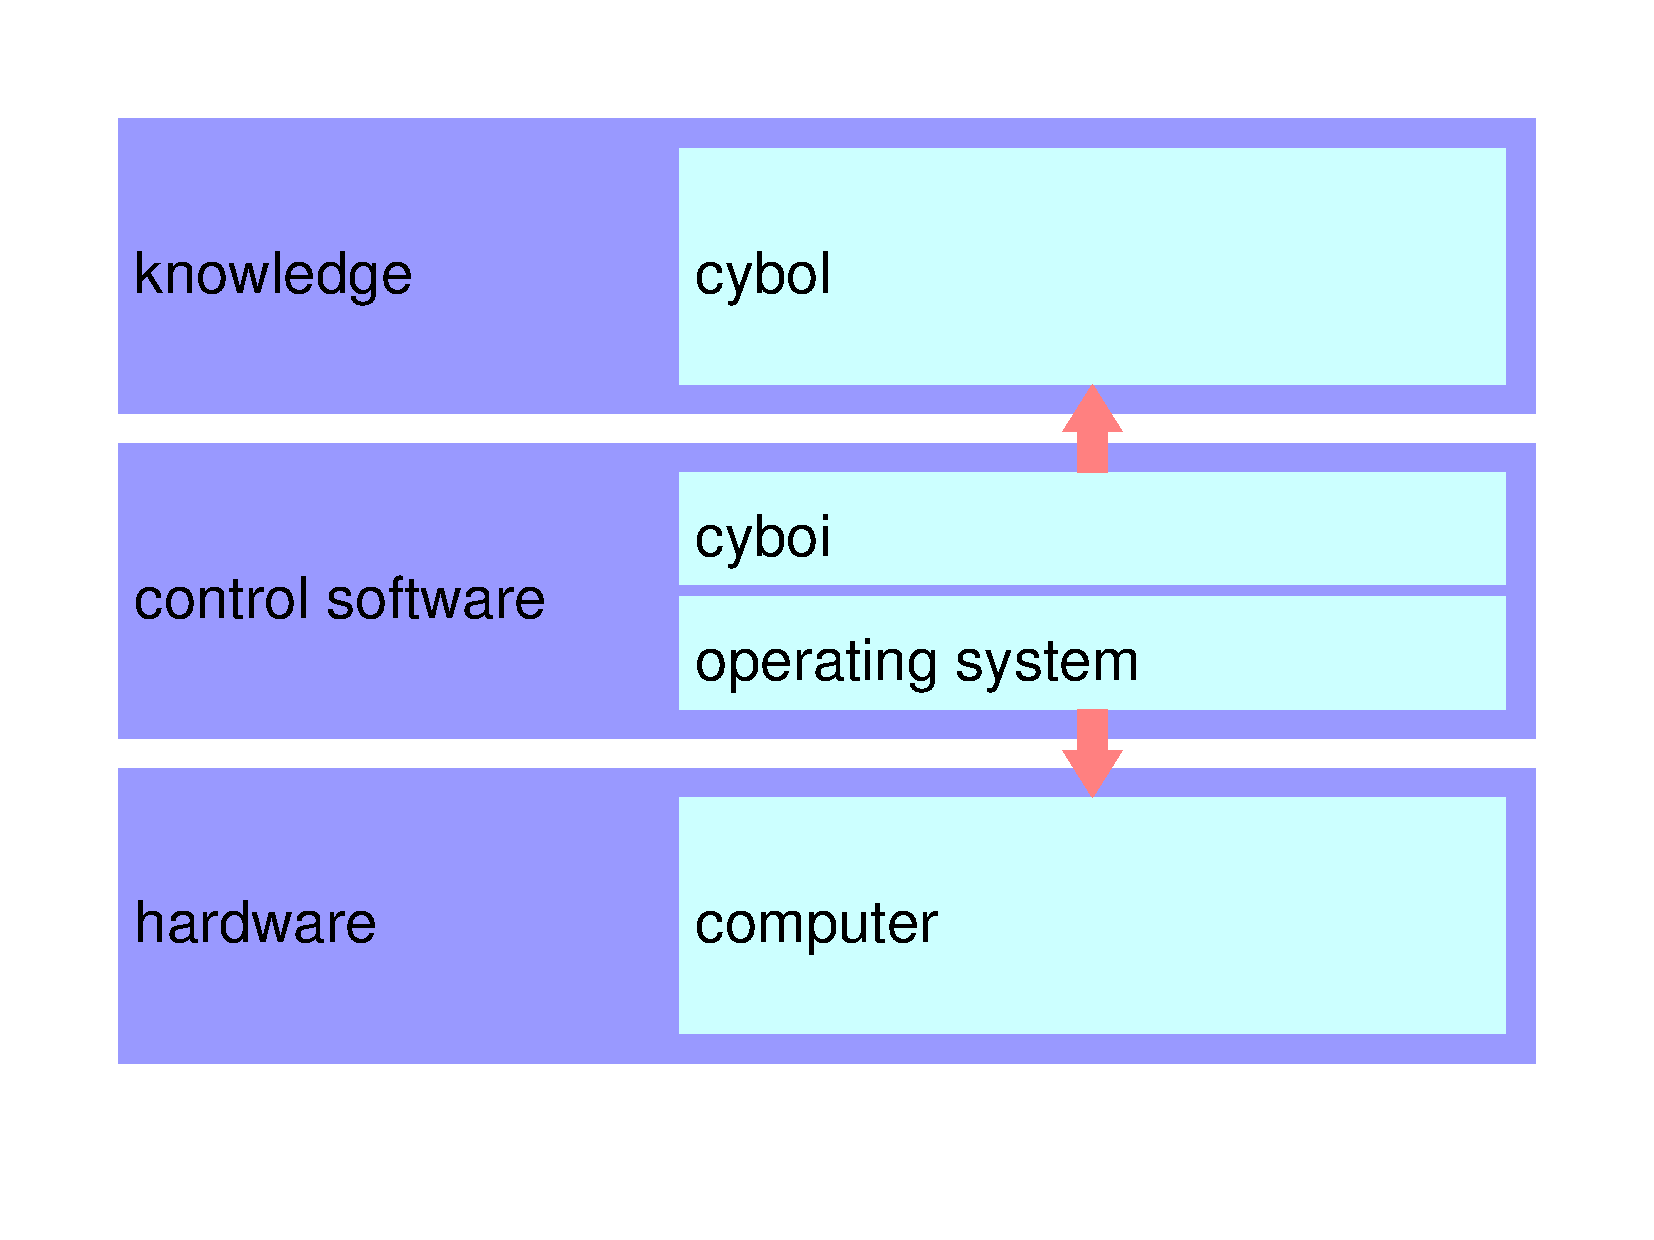
\includegraphics[scale=0.3,angle=-90]{graphic/connection.pdf}
        \caption{Knowledge -- Hardware Connection}
        \label{connection_figure}
    \end{center}
\end{figure}

Three main layers of information crystallise out: \emph{Knowledge},
\emph{Control Software} and \emph{Hardware} (figure \ref{connection_figure}).
Tanenbaum \cite{tanenbaum1999} calls the latter two \textit{logically equivalent}
(section \ref{paradigm_and_language_heading}), because one could replace the
other. It is indeed up to the computer designer to decide how much control
software should get burned into hardware. Hence, the important separation is
between \emph{Knowledge} on one side and \emph{Hardware} together with
\emph{Control Software} on the other.

The previous sections \ref{mind_and_body_heading}, \ref{brain_regions_heading}
and \ref{cell_division_heading} tried to justify this separation by looking at
nature. Knowledge is the equivalent of: \emph{Mind} (philosophically) and the
virtual information stored in a human brain's \emph{Hippocampus} and
\emph{Cerebral Cortex}, as well as of the information encoded in a biological
cell's \emph{Desoxy Ribo Nucleic Acid} (DNA). Hardware and control software are
the equivalent of: (philosophically) \emph{Body}, (neurologically) parts of the
human brain (\emph{Midbrain}, \emph{Basal Ganglia}) which coordinate the input/
output (i/o) of knowledge and (biologically) \emph{Ribo Nucleic Acid} (RNA)
molecules transmitting the genetic information from the DNA into proteins.

Chapters \ref{cybernetics_oriented_language_heading} and
\ref{cybernetics_oriented_interpreter_heading} will describe the
\emph{Cybernetics Oriented Language} (CYBOL) as knowledge specification format
and the \emph{Cybernetics Oriented Interpreter} (CYBOI) as system being able to
handle such knowledge, as well as to serve as hardware interface. All
hardware-controlling functionality needs to be present within either CYBOI or
the underlying \emph{Operating System} (OS) closely coupled with it. Together,
they are the active entity allowing virtual and real world (knowledge and
hardware) to communicate.

The remaining sections of this chapter describe important elements belonging to
a control software's architecture. More detailed descriptions of the
architecture and functionality will be given in chapter
\ref{cybernetics_oriented_interpreter_heading} devoted to CYBOI only.
